\theoremstyle{definition}
\newtheorem{definicion}{Definici\'on}

\begin{frame}
\titlepage
\end{frame}

\begin{frame}
\frametitle{A cubrir hoy\ldots}
\tableofcontents
% You might wish to add the option [pausesections]
\end{frame}
\section{Est\'andares relacionados con SCM}
\begin{frame}
	\frametitle{Sobre los standares (obligatory XKCD quote)}
	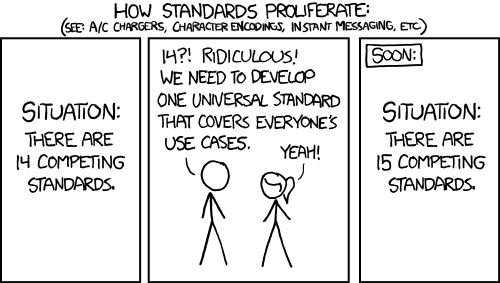
\includegraphics[scale=0.3]{standards.png}
\end{frame}
\subsection{Hist\'oria}
\begin{frame}
	\frametitle{El origen de los est\'andares de SCM}
	La idea de SCM se inicio en la industria de defensa de EUA. 
	\begin{itemize}
		\item La idea es evitar en dise\~nos que exista mala 
			calidad por malos componentes.
		\item En 1962 se desarrolla el CM-AFSCM 375-1. 
		\item De este se derivan varios otros (NASA/MIL/DOD)
		\item La mayor\'ia de los est\'andares militares fueron 
			sustituidos por est\'andares comerciales. 
        \end{itemize}
\end{frame}
\subsection{Est\'andares militares}
\begin{frame}
	\frametitle{Est\'andares militares}
	La mayor\'ia de los standares militares han sido supercedidos por 
	estandares comerciales. Funcionan como referencia his\'orica
	\begin{description}
		\item[DOD-STD-2167A] Desarrollo de software para defensa. Secci\'on 5 define las actividades de CM.
		\item[DOD-STD-2168] Documenta un plan de calidad para software. Especifica la parte de calidad del CM (Auditorias, revisiones, etc). 
		\item[MIL STD 973] Supercedido por EIA-649. Estandar militar de administraci\'on de configuraci\'on.
		\item[MIL STD 498] Supercedido por IEEE-12207. Define todas las actividades de desarrollo de software. 
	\end{description}
\end{frame}
\begin{frame}
	\frametitle{MIL-HDBK-61A (SE)}
	Manual militar MILHDBK-61A
	\begin{itemize}
		\item Da una descripci\'on detallada de c\'omo hacer 
			la planeaci\'on y administraci\'on de CM
		\item Tambi\'en una descripci\'on detallada de las actividades 
			del CM. 
	\end{itemize}
\end{frame}
\subsection{Est\'andares civiles y comerciales}
\begin{frame}
	\frametitle{Est\'andares civiles y comerciales}
	\begin{description}
		\item[IEEE-828] IEEE standard for CM. 
		\item[IEEE-1042] IEEE SCM guide. 
		\item[ANSI/EIA 649] CM Standard. 
		\item[ISO 10007] Quality management - guidelines for CM. 
	\end{description}
\end{frame}
\section{Modelos de mejora de procesos}
\begin{frame}
	\frametitle{CMM}
	\begin{itemize}
		\item Creado por el SEI
		\item Basado en la capacidad de la organizacion
		\item Habla de niveles de madurez de una organizacion:
			\begin{enumerate}
				\item Inicial
				\item Repetitivo
				\item Definido
				\item Administrado
				\item Optimizado
			\end{enumerate}
		\item Cada nivel se define por una serie de Areas de proceso
		\item CM es un proceso de nivel dos
	\end{itemize}
\end{frame}
\begin{frame}
	\frametitle{CM en CMM}
	Requiere que:
	\begin{itemize}
		\item Las actividades de CM estan planeadas.
		\item Los productos de trabajo de software estan identificados 
			controlados y disponibles.
		\item Los cambos son controlados
		\item Los grupos e individuos afectados son informados de 
			los cambios. 
	\end{itemize}
\end{frame}
\begin{frame}
	\frametitle{CMMi}
	Un modelo que incluye productos que no son de software. Combina SW-CMM, 
	SECM y IPD-CMM

	Puede ser continuo o por estados. 

	CM es un \'area de proceso de "soporte" que requiere:
	\begin{itemize}
		\item Establescer \emph{baselines}
		\item Seguir y controlar cambios
		\item Establescer integridad
	\end{itemize}


\end{frame}
\begin{frame}
	\frametitle{ITIL}
	Information Technology Infraestructure Library
	\begin{itemize}
		\item Orientado a IT: Las mejores pr\'acticas de IT. 
		\item Muy espec\'ifico para servicios. 
		\item Define el ciclo de vida del servicio, y las actividades
	\end{itemize}
\end{frame}
\begin{frame}
	\frametitle{ITIL y CM}
	\begin{itemize}
		\item Change evaluation
		\item Change management
		\item Release and delployment
		\item Service asset and CM
	\end{itemize}
\end{frame}

